
% This LaTeX was auto-generated from MATLAB code.
% To make changes, update the MATLAB code and republish this document.

\documentclass{article}
\usepackage{graphicx}
\usepackage{color}

\sloppy
\definecolor{lightgray}{gray}{0.5}
\setlength{\parindent}{0pt}

\begin{document}

    
    

\section*{22. Linear approximation: beyond polynomials}

\begin{verbatim}
ATAPformats
\end{verbatim}
\begin{par}

Several times in the previous chapters, we have hinted that polynomials
are not optimal functions for linear approximation on $[-1,1]$.  (Nonlinear
approximations are another matter and will make their appearance in the
next chapter.) It is now time to explain these hints and introduce
alternative approximations that may be up to $\pi/2$ times more
efficient. One reason the alternatives are valuable is that they have
practical advantages in some applications, especially for spectral
methods in more than one space dimension. An equally important reason is
that they push us to think more deeply about what it means to approximate
a function and what may or may not be special about polynomials. The
ideas of this chapter originate in [Bakhvalov 1967] and [Hale \& Trefethen 2008].
Related ideas
are the basis of work on sinc function numerical methods [Stenger 1993 \&
2010, Richardson \& Trefethen 2011],
tanh and double exponential or tanh-sinh quadrature [Sag \&
Szekeres 1964, Takahasi \& Mori 1974, Mori \& Sugihara 2001], and the
transformed-grid spectral methods introduced by Kosloff and Tal-Ezer
[1993].

\end{par} \vspace{1em}
\begin{par}
Recall from Chapter 8 that if $f$ is analytic on $[-1,1]$, then to investigate its polynomial approximations, we ask how large a Bernstein ellipse $E_\rho$ it can be analytically continued to. Here for example is the ellipse $E_\rho$ with $\rho=1.15$.  The words ``Bernstein ellipse'' written inside will help in a moment to visualize a conformal map. (Mathematically, these words are a piecewise linear complex function of a real variable constructed by the Chebfun \texttt{scribble} command.)
\end{par} \vspace{1em}
\begin{par}
 \vskip -2em 
\end{par} \vspace{1em}
\begin{verbatim}
x = chebfun('x'); w = exp(2i*pi*x);
z = @(rho) (rho*w+(rho*w).^(-1))/2;
clf, plot(z(1.15)), xlim([-1.1,1.1]), axis equal, grid on
FS = 'fontsize';
title('Bernstein ellipse for \rho=1.15',FS,9)
f = .01-.055i+.93*scribble('Bernstein ellipse');
hold on, plot(f,'k','linewidth',1.2)
\end{verbatim}

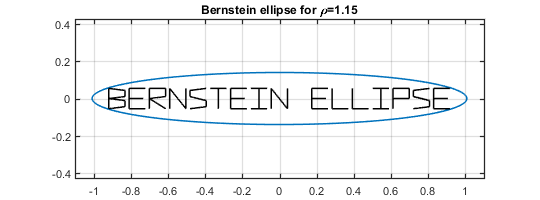
\includegraphics [width=4in]{chap22_01.png}
\begin{par}
 \vskip 1pt 
\end{par} \vspace{1em}
\begin{par}
Bernstein ellipses are unavoidable if one works with polynomial interpolants, but from the user's point of view, they have an unfortunate property: they are thicker in the middle than near the ends! For a function $f$ to be analytic in the region just shown, its Taylor series about a point $x\approx 0$ must have radius of convergence 0.14 or more. For $x\approx\pm 1$, on the other hand, a radius of convergence of 0.01 or less is sufficient. Thus the smoothness requirement on $f$ is highly nonuniform, and this is not an artifact of the analysis. Polynomials of a given degree really can resolve rougher behavior of a function $f$ near the endpoints than in the middle.  This phenomenon turns up in one form of another whenever approximation theorists seek sharp results about polynomial approximations, whether $f$ is analytic or not.  See for example [Timan 1951], [Lorentz 1986], [Ditzian \& Totik 1987], and Chapter 8 of [DeVore and Lorentz 1993].
\end{par} \vspace{1em}
\begin{par}

Of course, there are some functions that have most of their complexity
near $\pm 1$, and for these, the nonuniform approximation power of
polynomials may be an advantage. For example, functions of this kind
arise in fluid mechanics problems with boundary layers.  More often,
however, the nonuniform approximation power of polynomials is a
disadvantage from a practical point of view, as well as being a
conceptual complication.  If only those ellipses had constant width for
all $x\in [-1,1]\,$!

\end{par} \vspace{1em}
\begin{par}
As soon as one frames the difficulty in this way, a possibility for a solution suggests itself.  The idea is to change variables by means of a function that conformally maps ellipses, approximately at least, to straight-sided $\varepsilon$-neighborhoods of $[-1,1]$, while mapping $[-1,1]$ to itself. To explore this idea we shall use the variable $x$ for the domain where $f$ is defined and introduce a new variable $s$ for the parameter domain, where the Chebyshev points and ellipses live. Our conformal map will be $x = g(s)$, and we shall approximate a function $f(x)$ on $[-1,1]$ by $p(\kern .7pt g^{-1}(x)) = p(s)$, where $p$ is a polynomial. Equivalently, we shall approximate $f(\kern .7pt g(s))$ on $[-1,1]$ by a polynomial. In the remainder of this chapter we explore the consequences of this idea, considering just one fixed example of a map $g$, $$ g(s) = {1\over 53089}(40320 s + 6720 s^3 + 3024s^5 + 1800s^7 + 1225s^9), \eqno (22.1) $$ or as a Chebfun command,
\end{par} \vspace{1em}
\begin{par}
 \vspace{-2em} 
\end{par} \vspace{1em}
\begin{verbatim}
g = chebfun(@(s) (40320*s + 6720*s.^3 + 3024*s.^5 + ...
                           1800*s.^7 + 1225*s.^9)/53089);
\end{verbatim}
\begin{par}
This function $g$ is derived by truncating the Taylor series of $(2/\pi) \sin^{-1}(x)$ and then rescaling the result so that $g(\pm 1) = \pm 1$.  See [Hale \& Trefethen 2008] for a discussion of this and other possible choices of $g$, some of which (notably a conformal map onto an infinite strip) come closer to realizing the maximum possible improvement by a factor of $\pi/2$. See also Exercises 22.2 and 22.3.
\end{par} \vspace{1em}
\begin{par}
To begin the discussion, let us look at how $g$ transforms ellipses about $[-1,1]$.  Here is a plot of $g(E_{1.15})$, the transformed version of the ellipse shown earlier.  Notice the much straighter sides.
\end{par} \vspace{1em}
\begin{par}
 \vskip -2em 
\end{par} \vspace{1em}
\begin{verbatim}
hold off, plot(g(z(1.15)),'m')
xlim([-1.1,1.1]), axis equal, grid on
title('Transformation to a region with straighter sides',FS,9)
hold on, plot(g(f),'k','linewidth',1.2)
\end{verbatim}

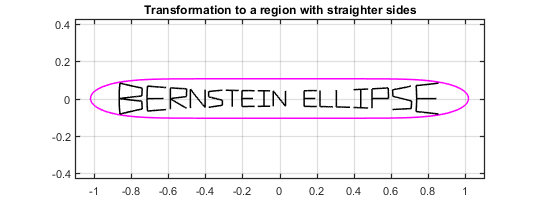
\includegraphics [width=4in]{chap22_02.png}
\begin{par}
 \vskip 1pt 
\end{par} \vspace{1em}
\begin{par}
Following [Hale \& Trefethen 2008], we call $g$ a \textit{sausage map} and $g(E_{1.15})$ a \textit{sausage region.} The crucial property is that for most of its length, the sausage is narrower than the ellipse, as the distorted ``Bernstein ellipse'' label makes clear. The ellipse has half-width approximately $\rho-1$, which is about $32\%$ more than the half-width $0.76\kern 1pt (\kern .7pt \rho-1)$ of the sausage:
\end{par} \vspace{1em}
\begin{par}
 \vskip -2em 
\end{par} \vspace{1em}
\begin{verbatim}
format short
ellipse_width = max(imag(z(1.15)))
sausage_width = max(imag(g(z(1.15))))
ratio = ellipse_width/sausage_width
\end{verbatim}

        \color{lightgray} \begin{verbatim}ellipse_width =
    0.1402
sausage_width =
    0.1061
ratio =
    1.3210
\end{verbatim} \color{black}
    \begin{par}
We can learn more by looking at a family of ellipses. Following Chapter 8, here is a plot of $E_\rho$ for $\rho= 1,1.2,\dots , 2.2$:
\end{par} \vspace{1em}
\begin{par}
 \vskip -2em 
\end{par} \vspace{1em}
\begin{verbatim}
w = exp(2i*pi*x); hold off
for rho = 1.1:0.2:2.2
    plot((rho*w+(rho*w).^(-1))/2), hold on
end
ylim([-1 1]), axis equal
title(['Bernstein ellipses in the s-plane'...
       ' for \rho = 1.1, 1.2, ... , 2.2'],FS,9)
\end{verbatim}

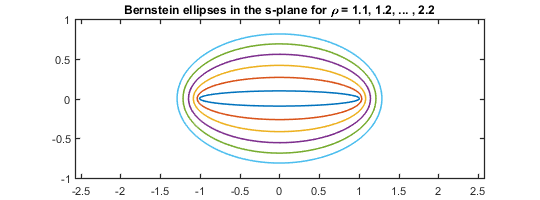
\includegraphics [width=4in]{chap22_03.png}
\begin{par}
 \vskip 1pt 
\end{par} \vspace{1em}
\begin{par}
Here is the corresponding figure for the images $g(E_\rho)$:
\end{par} \vspace{1em}
\begin{par}
 \vskip -2em 
\end{par} \vspace{1em}
\begin{verbatim}
hold off
for rho = 1.1:0.2:2.2
    plot(g((rho*w+(rho*w).^(-1))/2),'m'), hold on
end
ylim([-1 1]), axis equal
title('Transformed ellipses in the x-plane',FS,9)
\end{verbatim}

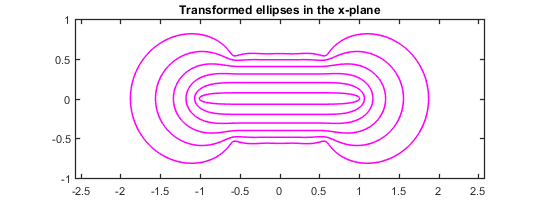
\includegraphics [width=4in]{chap22_04.png}
\begin{par}
 \vskip 1pt 
\end{par} \vspace{1em}
\begin{par}
It is clear that near $[-1,1]$, the transformed ellipses are narrower and more uniform in shape than the ellipses, but further away, their behavior is more irregular. We shall see some of the implications of these shapes as we explore the uses of this map.
\end{par} \vspace{1em}
\begin{par}
Chapter 2 considered polynomial interpolants in Chebyshev points $\{s_k\}$. With the transformation $g$, $f$ is interpolated by transformed polynomials $p(\kern .7pt g^{-1}(x))$ in the points $\{g(s_k)\}$.  We illustrate the difference between Chebyshev and transformed Chebyshev points by adapting a code segment from Chapter 17.  The squares show the transformed points.
\end{par} \vspace{1em}
\begin{par}
 \vskip -2em 
\end{par} \vspace{1em}
\begin{verbatim}
ss = chebpts(10);
clf, plot(ss,.9,'.b','markersize',8), hold on
plot(g(ss),.8,'sm','markersize',3)
ss = chebpts(20);
plot(ss,.5,'.b','markersize',8), plot(g(ss),.4,'sm','markersize',3)
ss = chebpts(50);
plot(ss,.12,'.b','markersize',8), plot(g(ss),0,'sm','markersize',3)
axis([-1 1 -.1 1.1]), axis off
\end{verbatim}

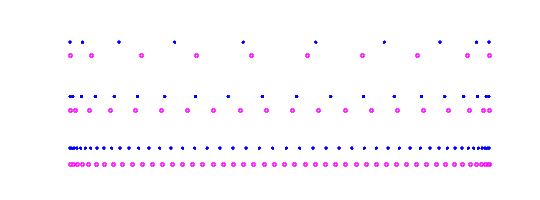
\includegraphics [width=4in]{chap22_05.png}
\begin{par}
 \vskip 1pt 
\end{par} \vspace{1em}
\begin{par}
Note that the squares are more evenly distributed than the dots, and in particular, they are denser in the middle, providing finer resolution.
\end{par} \vspace{1em}
\begin{par}
Chapter 3 considered Chebyshev polynomials and series.  We adapt another code segment from Chapter 17 to illustrate how a Chebyshev polynomial $T_n(x)$ compares to the corresponding transformed polynomial $T_n(\kern .7pt g^{-1}(x))$. For this we need the inverse map $g^{-1}$.
\end{par} \vspace{1em}
\begin{par}
 \vskip -2em 
\end{par} \vspace{1em}
\begin{verbatim}
gi = inv(g);
T50 = chebpoly(50); subplot(2,1,1), plot(T50), axis([-1 1 -2 2])
title('Chebyshev polynomial',FS,9), grid on, subplot(2,1,2)
plot(T50(gi),'m'), axis([-1 1 -2 2])
grid on, title('Transformed Chebyshev polynomial',FS,9)
\end{verbatim}

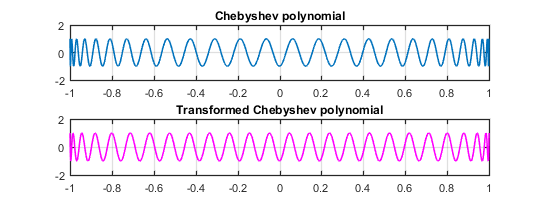
\includegraphics [width=4in]{chap22_06.png}
\begin{par}
 \vskip 1pt 
\end{par} \vspace{1em}
\begin{par}
Notice that the lower curves are more like uniform sine waves than the upper ones.
\end{par} \vspace{1em}
\begin{par}
Theorem 3.1 summarized some basic facts about Chebyshev series, and these carry over immediately to a theorem for transformed Chebyshev series. The theorem as stated assumes $g$ is analytic, though in fact, continuous differentiability would be enough.
\end{par} \vspace{1em}
\begin{par}
\textbf{Theorem 22.1. Transformed Chebyshev series.} \textit{Let $g$ be an analytic function on $[-1,1]$ mapping $[-1,1]$ to itself with $g'(s)>0$.  Then if $f$ is Lipschitz continuous on $[-1,1]$, it has a unique representation as an absolutely convergent series} $$ f(x) = \sum_{k=0}^\infty  a_k T_k(\kern .7pt g^{-1}(x)), \eqno (22.2) $$ \textit{and the coefficients are given for $k\ge 1$ by the formula} $$ a_k = {2\over\pi} \int_{-1}^1 {f(\kern .7pt g(s)) T_k(s)\over \sqrt{1-s^2}} ds, \eqno (22.3) $$ \textit{and for $k=0$ by the same formula with the factor $2/\pi$ changed to $1/\pi$.}
\end{par} \vspace{1em}
\begin{par}
\textit{Proof.} This is a consequence of Theorem 3.1. $~\hbox{\vrule width 2.5pt depth 2.5 pt height 3.5 pt}$
\end{par} \vspace{1em}
\begin{par}

For many functions $f$, the transformed series are $20$--$30\%$ more
efficient than the originals.  For example, Chebyshev interpolation of
$(2+\cos(20x+1))^{-1}$ requires about 520 terms for 15-digit accuracy:

\end{par} \vspace{1em}
\begin{par}
 \vskip -2em 
\end{par} \vspace{1em}
\begin{verbatim}
f = 1./(2+cos(20*x+1));
clf, chebpolyplot(f), grid on, axis([0 600 1e-18 1])
title('Chebyshev series coefficients',FS,9)
\end{verbatim}

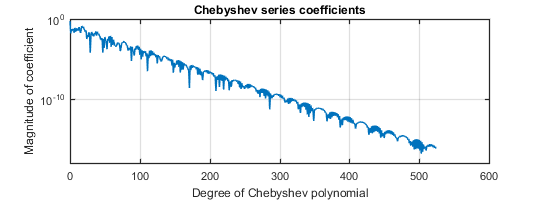
\includegraphics [width=4in]{chap22_07.png}
\begin{par}
 \vskip 1pt 
\end{par} \vspace{1em}
\begin{par}
For the transformed interpolants the figure is closer to 400:
\end{par} \vspace{1em}
\begin{par}
 \vskip -2em 
\end{par} \vspace{1em}
\begin{verbatim}
chebpolyplot(f(g),'m'), grid on, axis([0 600 1e-18 1])
title('Transformed Chebyshev series coefficients',FS,9)
\end{verbatim}

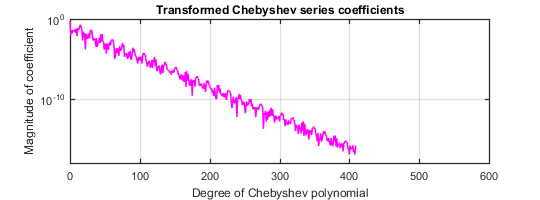
\includegraphics [width=4in]{chap22_08.png}
\begin{par}
 \vskip 1pt 
\end{par} \vspace{1em}
\begin{par}
Chapter 7 considered convergence for differentiable functions.  Theorem 7.2 can readily be restated for the transformed context---see Exercise 22.1.  For a numerical illustration, here is a repetition of the experiment from Chapter 7 involving $f(x) = |x|$.  On the loglog scale, the transformed approximants run parallel to the same line as the Chebyshev interpolants, but lower.
\end{par} \vspace{1em}
\begin{par}
 \vskip -2em 
\end{par} \vspace{1em}
\begin{verbatim}
f = abs(x); fg = f(g);
nn = 2*round(2.^(0:.3:7))-1; ee = 0*nn; ee2 = 0*nn;
for j = 1:length(nn)
    n = nn(j);
    fn = chebfun(f,n+1); ee(j) = norm(f-fn,inf);
    fn2 = chebfun(fg,n+1); ee2(j) = norm(fg-fn2,inf);
end
hold off, loglog(nn,1./nn,'r'), grid on, axis([1 300 1e-3 2])
hold on, loglog(nn,ee,'.'), loglog(nn,ee2,'sm','markersize',5)
ratio = ee(end-4:end)./ee2(end-4:end)
title(['Convergence of Chebyshev vs. '...
       'transformed Chebyshev interpolants'],FS,9)
\end{verbatim}

        \color{lightgray} \begin{verbatim}ratio =
    1.3167    1.3167    1.3167    1.3167    1.3167
\end{verbatim} \color{black}
    
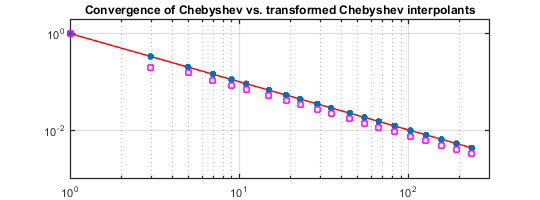
\includegraphics [width=4in]{chap22_09.png}
\begin{par}
 \vskip 1pt 
\end{par} \vspace{1em}
\begin{par}
Chapter 8 considered convergence for analytic functions. Here is the transformed equivalent of Theorems 8.1 and 8.2.
\end{par} \vspace{1em}
\begin{par}
\textbf{Theorem 22.2. Transformed coefficients of analytic functions.} \textit{For given $\rho>1$, let $g$ and $f$ be analytic functions on $[-1,1]$ that can be analytically continued to} $E_\rho$ \textit{and} $g(E_\rho)$, \textit{respectively, with $|f(z)|\le M$ for} $z\in g(E_\rho)$. \textit{Then the transformed Chebyshev coefficients of Theorem $22.1$ satisfy} $$ | a_k | \le 2M \rho^{-n}, \eqno (22.4) $$ \textit{the truncated transformed series satisfy} $$   \| f - f_n(\kern .7pt g^{-1}(x))\| \le {2M\rho^{-n}\over \rho - 1}, \eqno (22.5) $$ \textit{and the transformed Chebyshev interpolants satisfy} $$   \| f - p_n(\kern .7pt g^{-1}(x))\| \le {4M\rho^{-n}\over \rho - 1}. \eqno (22.6) $$
\end{par} \vspace{1em}
\begin{par}
 \vspace{-2em} 
\end{par} \vspace{1em}
\begin{par}
\textit{Proof.} These results follow from Theorems 8.2 and 22.1. $~\hbox{\vrule width 2.5pt depth 2.5 pt height 3.5 pt}$
\end{par} \vspace{1em}
\begin{par}
Here is a repetition of the Chapter 8 experiment for the Runge function, now with squares to show the transformed approximants.
\end{par} \vspace{1em}
\begin{par}
 \vskip -2em 
\end{par} \vspace{1em}
\begin{verbatim}
f = 1./(1+25*x.^2); fg = f(g);
nn = 0:10:200; ee = 0*nn; ee2 = 0:nn;
for j = 1:length(nn)
    n = nn(j);
    fn = chebfun(f,n+1); ee(j) = norm(f-fn,inf);
    fn2 = chebfun(fg,n+1); ee2(j) = norm(fg-fn2,inf);
end
hold off, semilogy(nn,ee,'.')
hold on, semilogy(nn,ee2,'sm','markersize',5)
grid on, axis([0 200 1e-17 10])
title(['Convergence of Chebyshev vs. '...
       'transformed Chebyshev interpolants'],FS,9)
\end{verbatim}

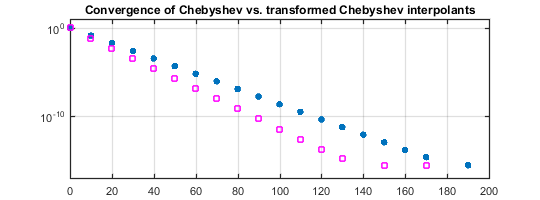
\includegraphics [width=4in]{chap22_10.png}
\begin{par}
 \vskip 1pt 
\end{par} \vspace{1em}
\begin{par}
The speedup is clear.  On the other hand, here is a repetition of the experiment with $\cos(20x)$.
\end{par} \vspace{1em}
\begin{par}
 \vskip -2em 
\end{par} \vspace{1em}
\begin{verbatim}
f = cos(20*x); fg = f(g);
nn = 0:2:60; ee = 0*nn; ee2 = 0:nn;
for j = 1:length(nn)
    n = nn(j);
    fn = chebfun(f,n+1); ee(j) = norm(f-fn,inf);
    fn2 = chebfun(fg,n+1); ee2(j) = norm(fg-fn2,inf);
end
hold off, semilogy(nn,ee,'.')
hold on, semilogy(nn,ee2,'sm','markersize',5)
grid on, axis([0 60 1e-16 100])
title(['Convergence of Chebyshev vs. '...
       'transformed Chebyshev interpolants'],FS,9)
\end{verbatim}

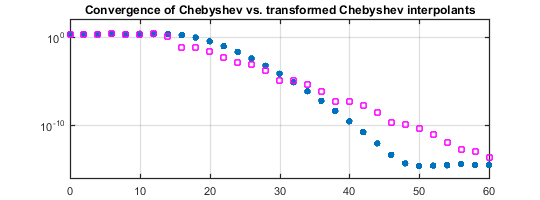
\includegraphics [width=4in]{chap22_11.png}
\begin{par}
 \vskip 1pt 
\end{par} \vspace{1em}
\begin{par}
Now the result is ambiguous: the transformed method starts out ahead, but the standard Chebyshev method wins eventually. The explanation can be found in the nested ellipses $E_\rho$ and their images plotted earlier. The function $\cos(20x)$ is entire, and for larger $n$, the Chebyshev points take good advantage of its analyticity well away from $[-1,1]$. The transformed points do not do as well. (The advantage of the transformation becomes decisive again if we change $\cos(20x)$ to $\cos(100x)$, at least down to 16-digit precision.)
\end{par} \vspace{1em}
\begin{par}
We can see similar effects if we look at best approximations. For a non-smooth function like $|x|$, transformed polynomials typically approximate better than true ones. The following figures should be compared with those of Chapter 10, and the variable \texttt{ratio} quantifies the degree of improvement.
\end{par} \vspace{1em}
\begin{par}
 \vskip -2em 
\end{par} \vspace{1em}
\begin{verbatim}
f = abs(x);
subplot(1,2,1), hold off, plot(f,'k'), grid on
fg = f(g);
[p,err] = remez(fg,4);
hold on, plot(p(gi),'m'), axis([-1 1 -.2 1.2])
title('Function',FS,9)
subplot(1,2,2), hold off
plot(g,f-p(gi),'m'), grid on, hold on, axis([-1 1 -.15 .15])
plot([-1 1],err*[1 1],'--k'), plot([-1 1],-err*[1 1],'--k')
[p2,err2] = remez(f,4); ratio = err2/err, title('Error curve',FS,9)
\end{verbatim}

        \color{lightgray} \begin{verbatim}ratio =
    1.2847
\end{verbatim} \color{black}
    
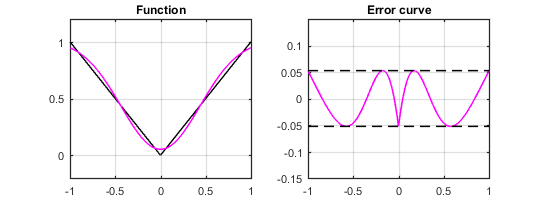
\includegraphics [width=4in]{chap22_12.png}
\begin{par}
 \vskip 1pt 
\end{par} \vspace{1em}
\begin{par}
On the other hand for a gentle entire function like $\exp(x)$, pure polynomials converge very fast and transformed polynomials cannot compete.  The following error curve is seven orders of magnitude larger than that of Chapter 10.
\end{par} \vspace{1em}
\begin{par}
 \vskip -2em 
\end{par} \vspace{1em}
\begin{verbatim}
f = exp(x);
fg = f(g);
[p,err] = remez(fg,10);
clf, plot(g,fg-p,'m'), grid on, hold on
plot([-1 1],err*[1 1],'--k'), plot([-1 1],-err*[1 1],'--k')
[p2,err2] = remez(f,10); ratio = err2/err
xlim([-1 1])
title('Error curve for best transformed approximation',FS,9)
\end{verbatim}

        \color{lightgray} \begin{verbatim}ratio =
   2.9938e-07
\end{verbatim} \color{black}
    
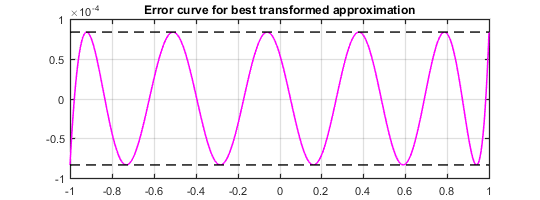
\includegraphics [width=4in]{chap22_13.png}
\begin{par}
 \vskip 1pt 
\end{par} \vspace{1em}
\begin{par}
Our final application of transformed polynomial approximants is the one that was the subject of [Hale \& Trefethen 2008]: quadrature.  As described in Chapter 19, standard quadrature formulas are based on the idea of integrating a function numerically by interpolating it by a polynomial, then integrating the interpolant.  This is the basis of all the well-known quadrature formulas, including Gauss, Newton--Cotes, Simpson, and Clenshaw--Curtis. But why should quadrature formulas be based on polynomials?  This is a question not often raised in the quadrature literature.  Some of the explanation surely has to do with custom going back centuries, before the appearance of computers, when the algebraic simplicity of polynomials would have been a telling advantage.  If one had to give a mathematical answer with still some validity today, it would probably be that a polynomial formula is optimal if the order is fixed while the grid size is decreased to zero. If the order increases to $\infty$ on a fixed interval of integration, however, polynomial formulas are in no sense optimal.
\end{par} \vspace{1em}
\begin{par}
In particular, a ``transformed Gauss'' quadrature formula can be obtained by applying Gauss quadrature to the integral on the right in the formula $$ \int_{-1}^1 f(x) = \int_{-1}^1 f(\kern .5pt g(s)) g'(s) ds. \eqno (22.7) $$ To illustrate this transplanted quadrature idea we pick a wiggly function,
\end{par} \vspace{1em}
\begin{par}
 \vskip -2em 
\end{par} \vspace{1em}
\begin{verbatim}
f = cos(17*x)./(1+sin(100*x).^2); clf, plot(f), ylim([-1.1 1.1])
title('A wiggly function','fontsize',9)
\end{verbatim}

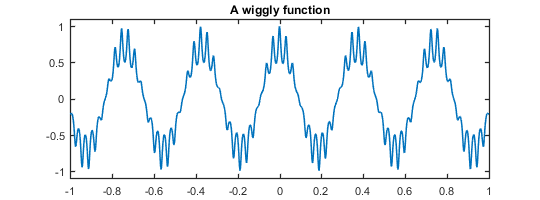
\includegraphics [width=4in]{chap22_14.png}
\begin{par}
 \vskip 1pt 
\end{par} \vspace{1em}
\begin{par}
Here is a code in which \texttt{I} represents Gauss quadrature and \texttt{I2} is transformed Gauss quadrature---and we see that the dots decrease about $30\%$ more slowly than the squares.
\end{par} \vspace{1em}
\begin{par}
 \vskip -2em 
\end{par} \vspace{1em}
\begin{verbatim}
gp = diff(g); Iexact = sum(f);
err = []; err2 = []; nn = 50:50:2000;
for n = nn
   [s,w] = legpts(n);
   I = w*f(s); err = [err abs(I-Iexact)];
   I2 = w*(f(g(s)).*gp(s)); err2 = [err2 abs(I2-Iexact)];
end
hold off, semilogy(nn,err,'.-','markersize',9), grid on
hold on, semilogy(nn,err2,'s-m','markersize',4), axis([1 2000 1e-16 1])
title('Convergence of Gauss vs. transformed Gauss quadrature',FS,9)
\end{verbatim}

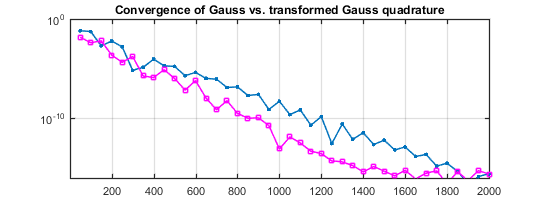
\includegraphics [width=4in]{chap22_15.png}
\begin{par}
 \vskip 1pt 
\end{par} \vspace{1em}
\begin{par}
We emphasize: in the end a quadrature formula is just a quadrature formula, as specified in (19.3): $$ I_n = \sum_{k=0}^n w_k f(x_k) . \eqno (22.8) $$ Gauss leads to one choice of nodes and weights, Clenshaw--Curtis leads to another, transplanted Gauss leads to a third, transplanted Clenshaw--Curtis to a fourth.  Regardless of what concepts may have been employed in the derivation, in the end the quadrature formula just takes a linear combination of function values, and the transformed formulas usually outperform the classical ones.  For example, in [Hale \& Trefethen 2008] it is proved that the transformed Gauss formulas based on mapping $E_{1.1}$ to an infinite strip converges $50\%$ faster than Gauss quadrature for the class of functions analytic in the $\varepsilon$-neighborhood of $[-1,1]$, for any $\varepsilon < 0.05$.
\end{par} \vspace{1em}
\begin{par}
This chapter has shown that polynomials are not the only effective general linear class of approximants for general functions $f$ on an interval and indeed are often suboptimal. There is much more that can be said on this subject. For example, there is the matter of how the mapping $g$ was derived and what other maps might be useful; an influential family of maps was introduced by Kosloff and Tal-Ezer [1993]. Another topic we have not discussed is the application to spectral methods, Kosloff and Tal-Ezer's motivation, and it is here that transformations of variables are perhaps most important in practice. Finally, there is the idea of using the map $g$ for rational functions rather than polynomials. The last two ideas have been combined powerfully in Tee's adaptive rational spectral collocation method based on adaptively determined conformal maps [Tee \& Trefethen 2006, Hale \& Tee 2009].
\end{par} \vspace{1em}
\begin{par}

\begin{displaymath}
\framebox[4.7in][c]{\parbox{4.5in}{\vspace{2pt}\sl
{\sc Summary of Chapter 22.}
Although many numerical methods are based on polynomial approximations of a
function $f\in C([-1,1])$, such approximations are not optimal in any
natural sense, for polynomials have higher resolution near the endpoints
of the interval than near the middle.  By a conformal transplantation one
can derive approximations that are up to $\pi/2$ times more
efficient.\vspace{2pt}}}
\end{displaymath}

\end{par} \vspace{1em}
\begin{par}
 \smallskip\parskip=2pt\small
\par
{\bf Exercise 22.1.  A challenging integrand.} Repeat the Gauss vs.\
transformed Gauss quadrature experiment for the ``challenging integrand''
(18.14). By approximately what percentage is Gauss slower than
transformed Gauss for this function?  How do you account for this
behavior?
\par
{\bf Exercise 22.2.  Chebfun 'map'.} Chebfun contains a \verb|'map'|
parameter that enables one to explore some of the ideas of this chapter
in an automatic fashion (try \verb|help maps| for information).
To illustrate this, construct \verb|f = 1./(1+25*x.^2)| with both
\verb|x = chebfun('x')| as usual and also
\verb|x = chebfun('x',|\verb|'map',|\verb|{'sausage',9})|.  How do the \verb|chebpolyplot|
results compare?  (b) What if the parameter 9 is varied to $1, 3, 5,
\dots 15$?  (This is the degree of the expansion in (22.1).)
\par
{\bf Exercise 22.3.  Transformed Clenshaw--Curtis quadrature.}
Generate the final plot of this chapter again, but now with two further
curves added corresponding to Clenshaw--Curtis and transformed
Clenshaw--Curtis quadrature.  How do the results compare with those
for Gauss and transformed Gauss?
\par
{\bf Exercise 22.4.  Gauss quadrature transformed by an infinite strip.}
Better than a sausage map for some applications is a map onto an infinite strip.
Following the last two exercises, use
\verb|x = chebfun('x',|\verb|'map',|\verb|{'strip',1.4})| to reproduce the
final plot of this chapter again, now with one other curve added corresponding
to Gauss quadrature transformed by the strip map of the Bernstein ellipse of
parameter $\rho=1.4$.  How do the results compare with those from the sausage transformation?
\par
{\bf Exercise 22.5.  Interpolation of equispaced data.}  Here is a scheme
for interpolation of data at equispaced points on $[-1,1]$:
use a conformal map $g^{-1}$ to transform the equispaced grid to an
approximate Chebyshev grid, and then compute a polynomial interpolant by
means of the barycentric formulas (5.11)--(5.12).  Explore this
method in Chebfun for interpolation of the Runge function $f(x) = 1/(1+25x^2)$
where $g$ is the map (22.1), using \verb|interp1| to compute the
interpolant.  Do these approximants weaken the Runge phenomenon?
(A theorem of [Platte, Trefethen \& Kuijlaars 2011] asserts that no approximation
scheme can eliminate the Runge phenomenon entirely.)

\end{par} \vspace{1em}



\end{document}
    
